\section{Vergleich von Java und Go}
\label{sec:Vergleich von Java und Go}

\subsection{Performancetest}
Die beiden Sprachen wurden mithilfe einer Testumgebung verglichen um Performanceunterschiede festzustellen. Die Testumgebung wurde folgendermassen aufgebaut.

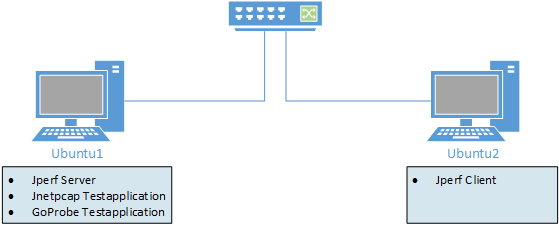
\includegraphics[width=0.7\textwidth]{start/img/PerformanceEvaluation.png}

Der Datenverkehr wurde mithilfe von Jperf simuliert und jeweil mit den beiden Testapplikationen aufgezeichnet.\\
Für Java wurde eine Testapplikation mit der Library JnetPcap erstellt. JnetPcap ist eine Opensource Library die einen wrapper für die Libpcap-Library zur verfügung stellt.\\
Für Go wurden die Pakete mithilfe von GoProbe aufgezeichnet. GoProbe ist ebenfalls Opensource und verwendet die Libpcap-Library.

\subsection{Performancetest Resultat}
Auslastung des Prozessors...